%%%%%%%%%%%%%%%%%%%%%%%%%%%%%%%%%%%%%%%%%%%%%%%%%%%%%%%%%%%%%%%%%%%%%%
%
% Preliminaries
%
%%%%%%%%%%%%%%%%%%%%%%%%%%%%%%%%%%%%%%%%%%%%%%%%%%%%%%%%%%%%%%%%%%%%%%

In this section we will introduce some background concepts about possibility theory and temporal databases. Subsection \ref{subsec:poss} is an introduction of possibility theory. The concepts defined by Dubois and Prade~\cite{Dubois1983} about fuzzy numbers and fuzzy intervals are also explained. Temporal databases and their characteristics are introduced in subsection \ref{subsec:temporal}.




\subsection{\label{subsec:poss}Possibilistic variables}
Informally, a theory of uncertainty considers a set of uncertain events and tries to quantify the confidence about the occurrence of those events. Consider therefore a set of outcomes $\Omega$ and let each subset of $\Omega$ be called an \emph{event}. Hereby, $\Omega$ is called the \emph{certain event} and can thus be regarded as a point of reference. Similarly, $\emptyset$ is called the \emph{impossible event}. The quantification of confidence in a theory of uncertainty is achieved by means of a \emph{confidence measure}~\cite{Choquet53}.
\begin{definition}
\label{def:conf-measure}
Consider a universe of outcomes $\Omega$. A confidence measure is defined by a function:
\begin{equation}
g:\Pow(\Omega)\rightarrow[0,1]
\end{equation}
that satisfies:
\begin{eqnarray}
g\left(\emptyset\right)&=&0\\
g\left(\Omega\right)&=&1\\
A\subseteq B&\Rightarrow&g(A)\leq g(B)
\end{eqnarray}
and where $\Pow(\Omega)$ represents the power set of $\Omega$.
\end{definition}
From the constraints in Definition \ref{def:conf-measure}, it can be seen that $\emptyset$ and $\Omega$ are indeed respectively the impossible and the certain event. In addition, the confidence that is assigned to events is monotonic. Due to this monotonicity, we have that:
\begin{eqnarray}
\forall A\in\Omega:\forall B\in\Omega&:&g\left(A\cup B\right)\geq\max\left(g\left(A\right),g\left(B\right)\right)\\
\forall A\in\Omega:\forall B\in\Omega&:&g\left(A\cap B\right)\leq\min\left(g\left(A\right),g\left(B\right)\right).
\end{eqnarray}
We can thus derive two extreme measures of confidence and these measures play a crucial role in the theory of possibility~\cite{Dubois88}. Consider a confidence measure $\Pi$ that satisfies the following constraint:
\begin{equation}
\label{EQ:MAXITIVITY}
\forall A\subseteq\Omega:\forall B\subseteq\Omega:\Pi\left(A\cup B\right) = \max\left(\Pi(A),\Pi(B)\right).
\end{equation}
The function $\Pi$ is then called a \emph{possibility measure} and due to \eqref{EQ:MAXITIVITY}, it is said that $\Pi$ is \emph{maxitive}~\cite{Dubois88}. For each event $A\subseteq\Omega$, $\Pi(A)$ expresses the possibility that $A$ occurs. Due to the maxitivity of $\Pi$ and under the constraint that $\Omega$ is finite, we can easily extract information about the possibility of separate outcomes in the form of a \emph{possibility distribution} $\pi$ defined by:
\begin{equation}
\pi:\Omega\rightarrow[0,1]:\pi(u)=\Pi\left(\left\{u\right\}\right).
\end{equation}
Equivalently, we have that:
\begin{equation}
\forall A\subseteq\Omega:\Pi(A)=\sup_{u\in A}\pi (u).
\end{equation}
A possibility distribution is normalized in the sense that:
\begin{equation}
\sup_{u\in\Omega}\pi(u)=1.
\end{equation}
In order to ensure the existence of a possibility distribution when $\Omega$ is infinite, the maxitivity constraint \eqref{EQ:MAXITIVITY} should be replaced by:
\begin{equation}
\Pi\left(\bigcup_{i}A_i\right)=\sup_{i}\Pi\left(A_i\right)
\end{equation}
for any family $\left\{A_i\right\}$ of indexed subsets of $U$~\cite{Nguyen79}.

Let us now consider a confidence measure $\N$ that satisfies:
\begin{equation}
\label{EQ:MINITIVITY}
\forall A\subseteq\Omega:\forall B\subseteq\Omega:\N\left(A\cap B\right) = \min\left(\Pi(A),\Pi(B)\right).
\end{equation}
The function $\N$ is then called a \emph{necessity measure} and due to \eqref{EQ:MINITIVITY}, it is said that $\N$ is \emph{minitive}. Possibility measures and necessity measures are dual in the sense that:
\begin{equation}
\forall A\subseteq\Omega:\Pi(A)=1-\N(\overline{A}).
\end{equation}
The principles of possibility theory are often used in the scope of a \emph{possibilistic variable}, also known as an \emph{ill-known value}.
\begin{definition}
Consider a universe $U$. A possibilistic variable $X$ over $U$ is a variable taking exactly one value in $U$, but for which this value is (partially) unknown. The available knowledge about the value that $X$ takes, is given by a possibility distribution $\pi_X$. For each $u\in U$, $\pi_X(u)$ represents the possibility that $X$ takes the value $u$.
\end{definition}
A specific application of possibility theory~\cite{Prade82,VanSchooten,DeCooman} is obtained when the universe is the set of Boolean values, i.e. $U=\mathbb{B}=\{T,F\}$. If we consider a Boolean proposition, then this proposition is either true ($T$) or false ($F$). Any Boolean proposition $p$ can thus be regarded as a possibilistic variable for which the possibility and necessity that $p=T$ are denoted in short as $\Pos(p)$ and $\Nec(p)$. The following notations are used:
\begin{eqnarray}
\Pos(p)&=&\pi_p(T)\\
\Nec(p)&=&1-\pi_p(F).
\end{eqnarray}
Keeping in mind the cause of uncertainty that is assumed, it is important to understand that a possibilistic variable $X$ is bounded to take one value only, but this value is not known due to incomplete knowledge. When a possibilistic variable is defined over the universe $\Pow(U)$, it is said to be a \emph{possibilistic multi-valued variable}, also known as an \emph{ill-known set}~\cite{Dubois88b}. Note that an ill-known set conceptually differs from a fuzzy set in the sense that an ill-known set is a crisp set, but for some reason (partially) unknown.
\subsection{\label{subsubsec:fuzzy}Fuzzy numbers and fuzzy intervals}
When we shall discuss the case of fuzzy temporal databases, we shall link the concepts introduced in this paper to the theory of fuzzy intervals. Dubois and Prade~\cite{Dubois1983} proposed the following definition of \emph{fuzzy interval}.
\begin{definition}
A fuzzy interval is a fuzzy set $M$ on the set of real numbers $\mathbb{R}$ such that:
\begin{eqnarray}
\forall (u,v)\in\mathbb{R}^2:\forall w \in [u,v]:&\mu_M(w) \geq\min(\mu_M(u),\mu_M(v)) \ &\mbox{ (convexity) } \\
\exists m \in \mathbb{R}:& \mu_M(m)=1 \ &\mbox{ (normalization) }
\end{eqnarray}
\end{definition}
If $m$ is unique, then $M$ is referred to as a \emph{fuzzy number}, instead of a \emph{fuzzy interval}. In other words, if the core of a fuzzy interval is a singleton, it can be seen as a fuzzy number. In their work, Dubois and Prade propose four different functions (two possibility and two necessity functions) to asses the position of a fuzzy number N relative to that of a fuzzy number M taken as a reference.

The most convenient representation for the membership function of a fuzzy number is a triangular function. The membership function $\mu_M$ for the fuzzy set $M$ has also the properties of convexity and normalization. Three values represent a triangular function (see Figure~\ref{fig:triangular}):
\begin{itemize}
\item
$D$ is the singleton value in the core of $\mu_M(x)$.
\item
$D-a$ is the lower value in the support of $\mu_M(x)$. 
\item
$D+b$ is the upper value in the support of $\mu_M(x)$.
\end{itemize}
Note that the values $a$ and $b$ are values in the underlying ordered domain. E.g. $(a,b) \in \mathbb{R}^2$. The notation for a triangular function adopted here is $[D,a,b]$.
\begin{figure}[h!]
  \centering
  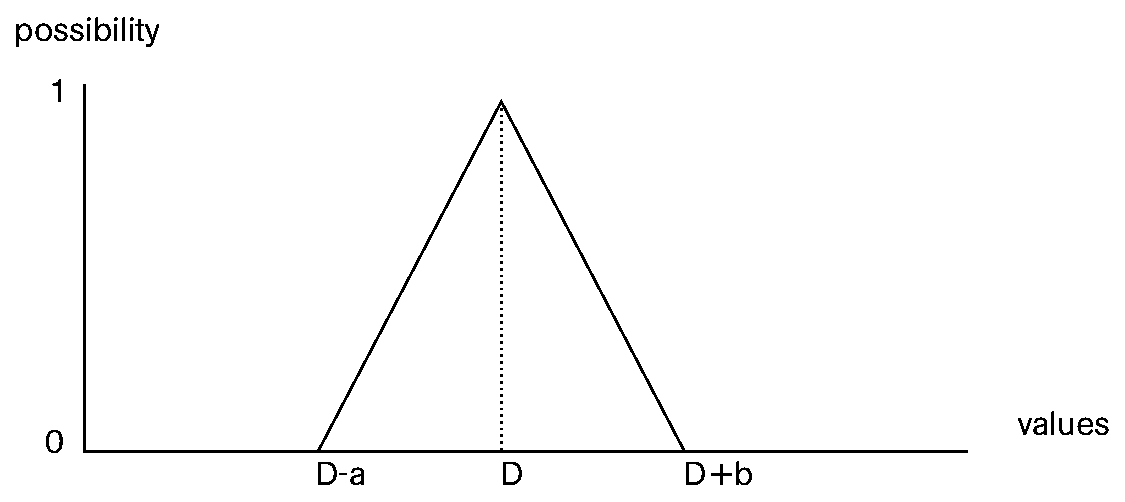
\includegraphics[scale=0.4]{graphs/triangular.eps}
  \caption{Triangular function.}
  \label{fig:triangular}
\end{figure}

The most simple representation for the membership function of a fuzzy interval is a trapezoidal function. This membership function $\mu_T$ for the fuzzy interval $T$ is convex and normalized. Four values represent a trapezoidal membership function (figure  \ref{fig:trapezoidal}): $\left[\alpha,\ \beta,\ \gamma,\ \delta\right]$. The membership function is given by:

\begin{align}
\mu_T(x)
\begin{cases}
1 & \mbox{ if } x \in [\beta,\gamma] \\
0 & \mbox{ if } x > \delta \vee x < \alpha \\
\frac{x-\alpha}{\beta - \alpha} & \mbox{ if } x \in [\alpha,\beta[ \\
\frac{\delta -x}{\delta - \gamma} & \mbox{ if } x \in ]\gamma,\delta] \\
\end{cases}
\end{align}

\begin{figure}[h!]
  \centering
  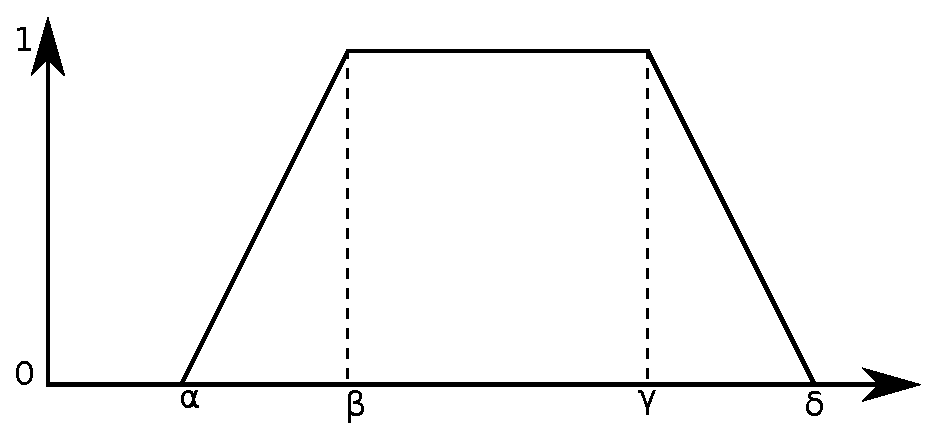
\includegraphics[scale=0.4]{graphs/trapezoidalDistribution.eps}
  \caption{Trapezoidal distribution.}
  \label{fig:trapezoidal}
\end{figure}






\subsection{\label{subsec:temporal}Temporal databases}

\subsubsection{\label{subsubsec:timeDomain}Time Domain}
The semantics of time and the different approaches to the time model are analyzed in this section; a more detailed explanation is discussed in \ref{sec:timeindatabasedesign}.

The general time model represents time as a set with an imposed partial order. There are two main models of time: linear and cyclic. In the linear model, time advances from the past to the future in a totally ordered fashion (a relationship of total order is imposed to the set). A cyclic model of time is used for recurrent processes. The present proposal focuses on the linear model.
\begin{itemize}
\item
Discrete model:  The discrete model of time is isomorphic in relation to the natural numbers. According to this model, each natural number corresponds to an indivisible time unit. The said time unit is called a chronon or, in other words, a 'time quantum', 'moment' or 'instant'. A chronon is the smallest time unit that can be represented by the model.
\item
Dense model: This model is isomorphic in relation to the rational or the real numbers. It represents one instant of time in the gap between another two instants.
\item
Continuous model: This is an extension of the dense model with no gaps. It is isomorphic in relation to the real numbers.
\end{itemize}
Restrictions on time range may be performed on the base of the following two concepts:
\begin{itemize}
\item
Time boundedness: Time can be bounded orthogonally in the past and in the future.
\item
Time distance: As a metric, time has a distance function which presents four properties:
\begin{enumerate}
\item
Distance is non-negative.
\item
The distance between two different elements is not equal to zero.
\item
The distance from $\alpha$ to $\beta$ is the same as that between $\beta$ and $\alpha$.
\item
Triangle inequality: The distance from $\alpha$ to $\gamma$ is equal or greater than the distance from $\alpha$ to $\beta$ plus the distance from $\beta$ to $\gamma$.
\end{enumerate}
\end{itemize}
On the other hand, time may be relative or absolute (in other words, anchored or unanchored). Sometimes, what one considers 'absolute time' is not as definite as one would hope since our concept of absolute time is based on another time reference (for example, January 1st of year one). Relative time has a direction, differently from distance. It is also possible to use negative references so as to represent relative time (e.g. -3 days = three days ago).

\subsubsection{Time in database design}
\label{sec:timeindatabasedesign}
This section defines the model used to represent time in a database. This model allows working with time instants and time intervals.  Even though there is no general agreement as to whether real-time line is continuous or discrete, a discrete model of time may be the most appropriate for a temporal database. 

	A chronon may be defined as the basic unit of time. Mathematically, a chronon is isomorphic to a finite sequence of natural numbers. For instance, if a chronon is \emph{11232010}, it represents a day, namely 11/23/2010. The symbol \emph{c} denotes a chronon. A chronon may represent different time granularity, depending on database or user processing needs (i.e. minutes, seconds, milliseconds, etc.). Real-time instants are smaller than chronons even though they are represented by the said chronons The real-time line is represented by a finite sequence of chronons. 

	It is possible to represent time intervals by a sequence of consecutive chronons. A sequence of consecutive chronons could be represented by the pair of starting and terminating chronons. A restriction must be imposed so that the starting instant comes before the ending instant.
\subsubsection{Temporal data models and time domains}
\label{sec:temporaldatamodelsandtimedomains}
A temporal data model is a relational data model which has temporal relations as underlying data structure, and whose operators are all temporal. In \cite{Böhlen_point-versus}, a study between interval-based and point-based temporal data models is shown. We are going to explain the main definitions and the equivalence between the models.

Temporal relations include a temporal attribute. A tuple of a temporal relation may be put under the form $(x_1,...,x_n||t_s)$ where $(x_1,...,x_n)$ are the non-temporal attribute values and \emph{t} is the tuple timestamp. Furthermore, an operator is temporal only if it generates a temporal relation when it is applied to temporal relations.

	The choice of the timestamp representation of the database facts is an important factor. Two options are the most common choices: time points and time intervals. Time intervals may be built from time points. The definition of time point is the following:
Let T be an infinite set.

$T^p=\langle T,< \rangle$ is a time point domain over $T$ iff $<$ defines a total order on $T$. Each element of $T$ corresponds to a time point of $T^p$.

The definition of time interval is:

A time interval $I$ of $T^p$ is any connected subset of $T^p$.

$T^i = \langle I,\subset \rangle $ is the time interval domain over $T^p$ iff $I$ is the set of all the intervals of $T^p$.

Both $T^p$ and $T^i$ are time domains over $T$.

A timestamp over $T^p$ is either a time point or a time interval of $T^p$. Time intervals can be represented as sets of time points which may, in turn, be represented by a time interval with the same values at both of its ends. Sometimes a coalesce operator is defined so as to switch between a set of time points and a time interval. Logically, defining a un-coalescing operator is quite complex. 
\subsubsection{\label{subsubsec:timeDb}Time in databases}
We can classify the time recorded in the database through its semantics. As a result, two kinds of time derive from two orthogonal time domains: valid time and transaction time. Valid-time captures the time-varying nature of the reality model. Transaction time structures the update activity associated with the object. The resulting temporal relations are those emerging from the bitemporal conceptual data model BCDM, on which TSQL2 is based.

The domain of valid time is given as $D_{VT}=\lbrace{c_1^v,c_2^v,...,c_k^v}\rbrace$, whereas the domain of transaction time may be given by $D_{TT}=\lbrace{c_1^t,c_2^t,...,c_k^t}\rbrace$. Thus, a valid-time chronon $c^v$  is a member of $D_{VT}$, a transaction-time chronon $c^t$ is a member of $D_{TT}$ and a bitemporal chronon $c^b=(c^t,c^v)$ is an ordered pair of a transaction-time chronon and valid-time chronon.

We can define the set of names $D_A=\lbrace{A_1,A_2,...,A_n}\rbrace$as attributes and the following set of domains for the said attributes:$D_D=\lbrace{D_1,D_2,...,D_n}\rbrace$. We may also define $\bot_i$ as inapplicable,$\bot_u$ as unknown, and $\bot$ as inapplicable or unknown null values. 

The schema for a bitemporal relation $'R'$ consists of an arbitrary number of explicit attributes from $D_A$ with domains in $D_D$ and an implicit timestamp attribute $T$ with domain $2^{\lbrace D_{TT}\bigcup \lbrace UC \rbrace \cdot D_{VT}\rbrace}$, where $UC$ ('until changed') means that the tuple is current in the database. This schema is a special transaction-time marker.

A 'fact' is the information stored in a tuple. We define a tuple as $x=(a_1,a_2,...,a_n|t^b)$ in a bitemporal conceptual relation instance $r(R)$, which consists of a number of attribute values associated with a bitemporal timestamp value. A value $(UC,c^v)$ in a timestamp indicates that the tuple is current in the database.

We say that a fact is true in the reality model during each valid-time chronon when a subset of the valid-time domain is associated with that fact.

We say that a fact is current in the relation during each transaction-time chronon when a subset of the transaction-time chronon domain is associated with the valid-time chronon. Only the subset of transaction times less than UC may be associated with a valid time.

While the definition of a bitemporal chronon is symmetric, the relation between valid time and transaction time is asymmetric. It should also be noted that since no two tuples with identical attribute values are allowed in a bitemporal relation instance, the full history of a fact is contained in a single tuple. In graphical representations of bitemporal space, the x-axis represents the transaction-time dimension and the y-axis denotes the valid-time dimension.

There are two special cases of bitemporal relations:
\begin{itemize}
\item
Valid-time relations, which support only valid time.
\item
Transaction-time relations,which support only transaction time.
\end{itemize}
We use the term 'snapshot relation' for a conventional relation. This relation supports neither transaction nor valid time.
\subsubsection{Implicit versus explicit timestamps}
\label{sec:implicitversusexplicittimestamps}
The association between time and facts may be carried out in two ways: explicitly, where the relation is represented by fully explicit timestamps, and implicitly. This distinction is relevant to three aspects of the data model: the update language, the display of data and the query language.

	If the time model works with transaction time, it means that the update language contains implicit timestamps. The transaction-time chronons of the facts are supplied by the system; in the valid-time model, these chronons are supplied by the user. Thus, in a bitemporal data model, the chronons are also supplied by the user.

	If the time model allows displaying temporal facts, it must represent such data explicitly. It is possible that the model allows the user to choose between several representations of time. In some simple transaction-time models it is common that the temporal facts cannot be displayed. 

	The main difficulty about differentiating between implicit and explicit timestamps is the query language. By means of the query language, we may directly access temporal attributes: the temporal attributes are as explicit as the other attributes in the database. If the query language does not allow direct access to temporal attributes, the association schema between timestamps and facts is considered implicit.
	
\subsubsection{\label{subsubsec:models}Temporal data models}
There are several extensions to the relational model that include the temporal element. In the current section, we briefly describe the model and some of its most interesting features. A more detailed summary can be found in \ref{sec:timeindatabasedesign}. Some models work only with valid or transaction time, whereas a few models can handle both. The current study starts with the models supporting valid time only, continues through the models which support transaction time and finally deals with the bitemporal models.

\paragraph{Valid-time models}
Most models support valid time only.

Brooks:  \cite{brooks56} Proposes a tridimensional view of valid-time database.

Wiederhold: \cite{Blum:1981:DCD:1672611.1672632} Time-oriented database, developed to work with medical applications. This model depicts relations as sets of entity-attribute-time-value quadruples. Time is associated with the visit number of the patient. 

Jones LEGOL 2.0: \cite{legol20} A language used in legislative writing. The temporal order of elements and the valid times for objects are important. It was the first time-oriented algebra to be defined, and some of its features are found in subsequent algebras.
Tuples in this model have two time attributes: Start and Stop. Each one indicates the start point and the end point of the interval where the tuple is valid.

Clifford-1: \cite{Clifford82},\cite{Clifford:1983:FST:319983.319986} Each relation schema has an additional time value called 'State'. Also, a boolean attribute is added to indicate if this tuple exists for that state.

Ariav: \cite{Ariav:1986:TOD:7239.7350} Temporally-oriented data model: a valid-time relation is a set of snapshot relation states indexed by valid time. A calculus-based query language is associated with the model: TOSQL.

Navathe: \cite{TSQL} Proposes a temporal extension to SQL called TSQL, the temporal algebra associated to the temporal relational model. This model allows a relationship to handle time-varying attributes, and also relationships without time-varying attributes. The only restriction is that all attributes in the relation must be of the same type. Objects are classified in snapshot relations and valid-time relations. In the latter, each tuple has associated to it an interval of validity with two points: time-start and time-end, like in the LEGOL 2.0 model.

Sadeghi: \cite{913787} Proposes a calculus-based valid-time language, HQL, where all objects represent valid-.time relations. As in Navathe and LEGOL 2.0, two time points are required for the ends of the interval. The model requires coalescing.

Sarda: \cite{Sarda:1990:ESH:627277.627409} This model was designed to support the calculus-based model HSQL. The model associates valid-time with tuples. Objects can either be snapshot or valid-time relations. In this model, valid time is considered to be closed on the left part of the interval and open on the right. Time is represented by an implicit attribute called 'Period' as a single non-atomic value.

The following time data models are not in first normal form (1NF), which means they might have multiple values per attribute. Even though these models are an extension of the 1NF, the representation is not in 1NF, but the operators work on valid-time relations, which are extensions of conventional relations.

Segev: \cite{Segev:1987:LMT:38714.38760} Defines the temporal data model, whose principal time structure is the time sequence. A time sequence is a surrogate value that identifies the object along with a sequence of time-value pairs. There are several types of time sequences depending on the semantics of the data represented. 

Clifford-2: \cite{Clifford:1987:HRD:645472.653241},\cite{Clifford:1985:AHR:971699.318922} This model is a refinement of the previous one presented by the same author. The data model allows two types of objects: a set of chronons, termed a lifespan, and a valid-time relation in which each attribute and tuple is assigned a lifespan. A tuple is an ordered value containing the tuple value and its lifespan. Attributes are not atomic since an attribute value in a tuple is a partial function from the chronons' domain to the value domain of the attribute. Relations have key attributes and, at the same chronon, no two tuples are allowed to match the key attributes.


Tansel: \cite{Tansel:1986:ATD:23125.23132},\cite{Clifford:1985:AHR:971699.318922} Designed to support the calculus-based query language (Hquel) and the time by example language. The model supports only one type of object: the valid-time relation. Four types of attributes are supported. If we take the time into account, attributes can be time-varying or non-time-varying. Then, attributes can be atomic-valued or set-valued. There is no need for attributes in the relation to be of the same type, and attribute values in a given tuple do not need to be homogeneous. A triplet containing an element from the attribute's value domain and the boundary points of the time interval represents the value of a time-varying atomic-valued attribute. A set-valued attribute is represented by a set of these triplets.

Gadia-1:  \cite{Gadia:1988:HRM:49346.50065},\cite{Gadia:1985:QLH:325405.325412} This homogeneous model allows two types of objects: valid-time elements and valid-time relations. The model requires that all attribute values in a given tuple be functions on the same valid-time element. Unlike intervals, valid-time elements are closed under union, difference, and complementation.
Bhargava presents an extension of this model to both valid and transaction time. 

Gadia-2: \cite{Gadia:1986:TMM:645471.655410},\cite{Chuen},\cite{Gadia:1988:GMR:971701.50233} Is an extension of the homogeneous model known as multihomogeneous model. Temporal elements may be multi-dimensional to model both valid and transaction time. Attribute values are functions from temporal elements onto attribute value domains, but attribute values do not need to be on the same temporal element. The key attributes in the relations must be single-valued in respect to the interval of validity. 

Lorentzos: \cite{springerlink:10.1007/3-540-19074-0_71},\cite{Lorentzos:1989:HDT:70777.70787} The temporal relational model allows to specify different granularities and the support of periodic events. This model associates timestamps with individual attribute values rather than with tuples. Timestamps are explicit values updated directly by the user. The said timestamps represent either the chronon during which attribute(s) were valid or a boundary point of the interval of validity. In the model, several timestamps of different granularities can be used together in the specification of a chronon.
This model has the particularity that some columns have a different meaning depending on the context.

\paragraph{Transaction-time models}
The main feature of the transaction-time models is that they are append-only.

Kimball: \cite{kim78} The temporal model is called DATA. In it, the association between facts and times is implicit. Also, the update operations avoid the explicit use of time. However, transaction-time relations cannot be displayed but can only be depicted in the snapshots extracted from the transaction-time relations. At query language level, the association of facts and times is also implicit.

Stonebraker: \cite{Ston87} Proposes the Postgres data model. Like in the previous model, the association between time and facts in the three model features (update language, query language and visualization) is implicit. In this model, the visualization is not restricted to snapshot relation states.
In this model, two timestamps are used when specifying the time for a given tuple that is current in the relation.

Jensen: \cite{Jensen:1991:IIM:627283.627484} In the DM/T model, the association of facts and times is also implicit. DM/T contains a backlog for each user-defined transaction-time relation. This backlog contains the full history of the associated user-defined transaction-time relation. When an insert, delete or update operation is performed, the backlog for this relation is updated.

\paragraph{Bitemporal data models}
The bitemporal data models support both valid and transaction time. This section deals with the following seven models of a bitemporal data model.

Ben-Zvi: \cite{910377} Proposed the time relational model,, which defines two types of objects: snapshot relations and bitemporal relations. Each tuple in a bitemporal relation has five additional implicit attributes:
The two interval ends of the valid-time chronon, called 'Effective-time-start' and 'Effective-time-stop'.
The two interval ends of the transaction-time chronon. 'Registration-time-start' is the transaction-time chronon associated with the 'Effective-time-start', 'Registration-time-stop' is the transaction-time chronon associated with the 'Effective-time-stop'.
Deletion-time. It registers when a tuple which was mistakenly entered is logically deleted.

Ahn: \cite{Snodgrass:1985:TTD:318898.318921},\cite{sno86} This model follows a four-dimensional data model. Each instance is represented as a sequence where each value is composed by a timestamp with a transaction-time chronon and a three dimensional volumes -one of these dimensions being the valid time.

Snodgrass:  \cite{sno86},\cite{Snodgrass:1984:TQL:588011.588041} The data model has four implicit attributes: 
The transaction time when the tuple was inserted.
The transaction time when the tuple was deleted.
The starting point of the valid-time interval.
The end point of the valid time-interval.
	
	The data query language associated with the model is called TQuel.

McKenzie: \cite{Snodgrass:1993:ATQ:642875.642890},\cite{Mckenzie:1988:ALQ:915060}, \cite{mck81} In this model, the attribute's values are timestamped, but it is required that attributes be single-valued. This makes it possible to perform a Cartesian product. There are two types of objects in the model: the snapshot relations and the valid-time relations. Thus, transaction-time relations are modeled as sequences of snapshot relations. Bitemporal relations are sequences of valid-time relations indexed by transaction time. An attribute's value in a valid-time relation is an ordered pair: a value from the attribute's domain and a set of chronons. Relations are not allowed to have value-equivalent tuples. The model also allows the schema and even the class of the relation (snapshot, transaction-time, valid-time and bitemporal) to change.

Gadia-3: \cite{Bhargava:1993:RDS:642811.642819},\cite{gad92} This data model is associated with the calculus-based query language TempSQL. Attributes are timestamped with finite unions of rectangles in the valid-time x transaction-time space.

Thompson: \cite{171833} This model, based on an accounting system, is called Accounting Data Model. It has four timestamp attributes: two for transaction time, called 'engineering time', and two for valid time, called 'accounting time'. Also, a boolean value called 'timewarp' enables the attribute to change historically. 

